\documentclass[tikz,border=2mm]{standalone}

\usepackage{rotating}

\tikzset{every picture/.style={line width=2pt},
        arcWeight/.style={midway, fill=white, scale=0.75, rotate=-45, text=black}}

\begin{document}

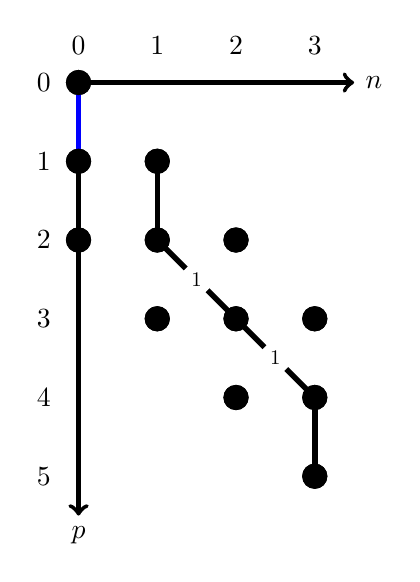
\begin{tikzpicture}

% draw axis and grid
\draw[->,ultra thick] (0,0)--(3.5,0) node[right]{$n$};
\draw[->,ultra thick] (0,0)--(0,-5.5) node[below]{$p$};

\foreach \i in {0,...,3} {
    \node[circle, label=above:\i] at (\i,0) {};
}

\foreach \i in {0,...,5} {
    \node[circle, label=left:\i] at (0,-\i) {};
}

%\draw[help lines, color=gray!30, dashed] (0,0) grid (4,-6); % uncomment this if you want a grid

% draw nodes
\foreach \i in {0,...,3} {
    \node[circle, draw=black, fill=black, scale=0.75] (i-\i) at (\i, -\i) {};
    \node[circle, draw=black, fill=black, scale=0.75] (j-\i) at (\i, -\i-1) {};
    \node[circle, draw=black, fill=black, scale=0.75] (k-\i) at (\i, -\i-2) {};
}

% draw necessary paths
\draw[blue] (i-0) -- (j-0);
\draw (i-1) -- (j-1);
\draw (j-1) -- (j-2) node[arcWeight] {\rotatebox{45}{1}};
\draw (j-2) -- (j-3) node[arcWeight] {\rotatebox{45}{1}};
\draw (j-3) -- (k-3);

% draw nodes such that lines don't go over nodes
\foreach \i in {0,...,3} {
    \node[circle, draw=black, fill=black, scale=0.75] (i-\i) at (\i, -\i) {};
    \node[circle, draw=black, fill=black, scale=0.75] (j-\i) at (\i, -\i-1) {};
    \node[circle, draw=black, fill=black, scale=0.75] (k-\i) at (\i, -\i-2) {};
}

\end{tikzpicture}
\end{document}